\documentclass{article}
\usepackage{amsmath,graphicx,amsfonts,amssymb,amsthm,hyperref,amscd}
\setcounter{MaxMatrixCols}{30}
\usepackage{tikz-cd}
\setcounter{tocdepth}{10}
\providecommand{\U}[1]{\protect\rule{.1in}{.1in}}
\setlength{\topmargin}{-1.0in}
\setlength{\textheight}{9.25in}
\setlength{\oddsidemargin}{0.0in}
\usepackage{mathtools}
\setlength{\evensidemargin}{0.0in}
\setlength{\textwidth}{6.5in}
\def\labelenumi{\arabic{enumi}.}
\def\theenumi{\arabic{enumi}}
\def\labelenumii{(\alph{enumii})}
\def\theenumii{\alph{enumii}}
\def\p@enumii{\theenumi.}
\def\labelenumiii{\arabic{enumiii}.}
\def\theenumiii{\arabic{enumiii}}
\def\p@enumiii{(\theenumi)(\theenumii)}
\def\labelenumiv{\arabic{enumiv}.}
\def\theenumiv{\arabic{enumiv}}
\def\p@enumiv{\p@enumiii.\theenumiii}
\pagestyle{plain}
\parindent=0pt
\newcommand{\Z}{\mathbb{Z}}
\newcommand{\B}{\beta}
\newcommand{\A}{\alpha}
\newcommand{\N}{\mathbb{N}}
\newcommand{\Ha}{\mathbb{H}}
\newcommand{\C}{\mathbb{C}}
\newcommand{\R}{\mathbb{R}}
\newcommand{\F}{\mathbb{F}}
\newcommand{\Q}{\mathbb{Q}}
\newcommand{\Oa}{\mathcal{O}}
\newcommand{\K}{\mathcal{K}}
\newcommand{\as}{\text{*}}
\newcommand{\tr}{\text{tr}}
\newcommand{\dt}{\bullet}

\newtheorem{theorem}{Theorem}[subsection]
\newtheorem{exercise}[theorem]{Exercise}
\newtheorem{example}[theorem]{Example}
\newtheorem{corollary}[theorem]{Corollary}
\newtheorem{lemma}[theorem]{Lemma}
\newtheorem{proposition}[theorem]{Proposition}
\theoremstyle{definition}
\newtheorem{definition}[theorem]{Definition}
\newtheorem{remark}[theorem]{Remark}
\newtheorem*{claim}{Claim}
\newtheorem{axiom}{Axiom}

\usepackage[english]{babel}
\usepackage[utf8]{inputenc}

\usepackage{caption}
\usepackage{subcaption}
\usepackage{wrapfig}

\title{Space Junk Research Notes}
\date{}
\author{Felipe}
\begin{document}
\maketitle 

Debris FAQ \cite{debrisFAQ}.
\linebreak
Acronyms:
\begin{itemize}
  \item LEO = Low Earth Orbit
  \item OP = Orbital Plane
\end{itemize}

ToSite:
\begin{enumerate}
  \item http://www.orbitaldebris.jsc.nasa.gov/library/IAR\_95\_Document.pdf 
  \item http://ccar.colorado.edu/asen5050/projects/projects\_2003/wilson/
  \item National Research Council Staff. Orbital Debris : A Technical Assessment. Washington, DC, USA: National Academies Press, 1995. ProQuest ebrary. Web. 28 January 2016.
  \item https://fas.org/irp/agency/dod/jason/leo.pdf
  \item http://www.esa.int/Our\_Activities/Operations/Space\_Debris/About\_space\_debris
  \item http://www.globalcomsatphone.com/hughesnet/satellite/altitudes.html
  \item http://www.nap.edu/read/4765/chapter/4\#23
\end{enumerate} 

\section{Future Directions}
There are three components, in our opinion, that would make our debris model much stronger.

\begin{enumerat}
	\item \textbf{Support for variable Debris Size: }Space Debris can be categorized in small (<1cm), medium (1-10cm) and large (>10cm). The number of each of these debris fragments greatly between categories and pose different kinds of threats to operational spacecrafts. Small particles can produce more small particles when colliding with spacecrafts or large-sized debris. Medium-sized can produce breakups or even explosions in operational spacecrafts. Finally, large debris fragments have the highest probability of destroying operational spacecrafts upon collisions. Therefore, this would be a very important step to a precise characterization of space debris.
	\item \textbf{Validation of Data: }All of the data used during initialization and throughout the time evolution was obtained from reputable sources. Being able to validate that the data we are using in our model would be highly beneficial. Numbers such as the initial debris concentration, or the altitudes spacecrafts are being launched, or the amount of mission-related debris could always be validated. This would make our model more robust.
	\item \textbf{Evaluation of more Debris Removal Strategies: } Our model determined that if we are able to remove a certain amount of debris per day we can prevent LEO debris to reach the critical mass described in Kessler's Syndrome. Therefore, the next step is to further quantitatively evaluate debris removal technologies and determine the most effective and economically feasible strategy.  
\end{enumerate}

\section{Model 3: Space Launches}

Building upon Model 2 we introduced yearly LEO spacecraft launches as stochastic events. These events will introduce a satellite to one of the levels in LEO and a constant amount of debris to that same level. There were three main components that we had to figure out in order to incorporate spacecraft launches into our model.

\textbf{Target Level: }In order to determine which level of our model a launch would arrive to, we looked at the Space Launch Report yearly log files \cite{spaceLaunchReport}. First, we looked at the log files from 2000-2015 to calculate the average launches to LEO. Then we looked at how these launches were categorized in the log files. These were: LEO/ISS, LEO/SS-O, and LEO (which we refer to as LEO/Other). Using data from 2010-2015 we calculated the average number of launches to each of these categories (ISS, SS-O and Other). The third step was to calculate the ratio of how many of the total number of launches in a year go into each of the three possible categories. The calculated ratios can be found in \ref{launchRatios}.  Finally using the determined target place we could determine the altitude by generating a uniform random variable between the altitude ranges in table \ref{altitudeRanges}.  
\begin{table}[h]
\centering
    \begin{tabular}{| c | c | c | c |}     
    \hline
    \textbf{\shortstack{Avg. LEO Launches \\ Per Year}} & \textbf{Ratio of LEO/ISS} & \textbf{Ratio of LEO/S}  & \textbf{Ratio of LEO/Other}\\ \hline
    36.4375 & 0.2850 & 0.3842 & 0.3308\\ \hline
	\end{tabular}
\captionof{table}{Calculated ratios from data in Appendix .}
\label{launchRatios}
\end{table}

\begin{table}[h]
\centering
    \begin{tabular}{| c | c | c |}     
    \hline
    \textbf{LEO/ISS (km)} & \textbf{LEO/SS-O (km)} & \textbf{LEO/Other (km)} \\ \hline
    $370-460$ & $600-800$ & $200-1600$ \\ \hline
	\end{tabular}
\captionof{table}{Altitude ranges used to determine which level a given launch ends up in. ISS range was obtained from \cite{esaISS} and SS-O range was determined by noticing that the largest number of operational satellites orbit at those altitudes.}
\label{altitudeRanges}

\end{table}

\textbf{Launch Rate Per Level: } In order to determine the launch rate, and incorporate as a stochastic event we used the results from determining the target level. Every 365 days we would generate a distribution of launches to each level using the data and results from the target level section . Using this distribution we could calculate the launch rates per level for the following year.

\textbf{Amount of released debris: }Our model takes the amount of debris released per launch as a constant. We set this constant to $70$ because according to \cite{orbitalDebris} a detailed study of a Russian launch mission determined that $76$ different objects were put into orbit.


\section{Background}\label{Background}

Since the launch of Sputnik in 1957 the number of artificial objects orbiting the Earth has been steadily increasing. In 1978, Donald Kessler of NASA hypothesized that there exists a critical mass for space debris, above which the frequency of collisions and creation of new debris would cascade and Earth's orbital space would become too densely filled with debris for space travel to be feasible. Thousands of spacecrafts have been sent into orbit, from which as of 2015, 696 are operational \cite{satelliteDB}, making the rest of them space debris. Space debris is not only constituted by nonfunctional spacecrafts, as shown in Figure \ref{fig:classesOfSpaceObjects}. Note that most of the objects in Figure \ref{fig:classesOfSpaceObjects} are either released at the beginning of a mission (after launch), during the lifetime of a satellite or the end of life of the satellite (breakups and/or malfunctions) \cite{orbitalDebris, studyOfOrbitalDebris}. If the combination of all of these space travel related objects is not controlled in someway, Donald Kessler hypothesis poses a big threat to space travel in the future.



\section*{Assumptions}
\begin{enumerate}
  \item Spacecrafts and satellites in MEO and GEO have extremely low probabilities to be affected by the amount of debris in those orbits. Therefore, debris removal strategies should only target LEO.
  \item The number of LEO launches per year is constant. This constant was obtained from the average number of LEO launches from 2010-2016.
  \item The fraction of the total number of launches per year that go to the ISS (370-460) to the Sun Synchronous Orbit (SS-O) (600-800) and to Other altitudes (200-1600) in  LEO is constant. This constant fractions from the total number of launches were calculated using the number of launches from 2010-2015 to these altitudes.
  \item The altitudes for yearly missions to the ISS are uniformly distributed between 370-460km. The same goes to missions to SS-O and Other.
  \item The amount mission-related debris is constant across missions, and all of the debris released by the mission is dropped at the altitude where the mission ends. For example, a mission going to the ISS will drop all of the debris somewhere between 370-460 km.
  \item The amount of debris obtained from figure  at a certain level is uniformly distributed throughout the level. 
  

\end{enumerate}
\section*{Systematic Production}

We are going to define the term Systematic Production  as the debris production due to space assets: i.e satellites, rockets, space stations, humans, etc.

\begin{itemize}
  \item At launch rocket bodies are left orbiting the earth. These create multiple kind of debris: motor casings, aluminum oxide exhaust particles, nozzle slag, and solid fuel fragments. Basically a lot of stuff is freed in the early life of the spacecraft. [2]
  \item As the spacecraft is subjected to solar heating, solar radiation, and atomic oxygen material degradation begins to free small particles of paint and multi-layer insulation [2]
  \item Towards the end of life object breakup becomes a possibility. This can be due to a collision or explosion [2].
  \item Most spacecrafts that reach their end of life (EOL), either through termination or malfunction are left in orbit.[3]
\end{itemize}

This will be highly dependent on the rate of spacecraft launches. A log of the number of space launches is kept in the Space Launch Report \cite{spaceLaunchReport}. We want to determine the distribution of LEO altitudes at which these spacecrafts end up. To this end, it is important to note that LEO altitude is usually determined by a target orbit lifetime, $t_{orbit}$ [4]. Depending on the function of the satellite the altitude is chose accordingly. According to [6] these are:

\begin{itemize}
  \item 300-600mi: Observation satellites used for photography, mapping, and environmental observations.
  \item 300-600mi: Search-and-rescue satellites also belong to this orbit. They are used to transmit emergency radio signals in case of an emergency.
  \item 3,000mi: Science satellites
  \item 6,000: GPS satellites
  \item Geostationary: Weather satellites, and communication satellites
  \item ISS orbital altitude range = [370km, 460km] \cite{esaISS}
  \item
\end{itemize}




\subsection*{Mission-related Debris}
Everything in this section was obtained from book [7].
The majority of functional spacecraft are accompanied into Earth orbit by one or more stages (or "rocket bodies") of the vehicles that launched them. 

\begin{itemize}
  \item Usually \textbf{1} rocket body is left in LEO.
  \item high-altitude spacecraft such as GOES (Geostationary Operational Environmental Satellite) may release up to three separate rocket bodies in different orbits along the way to its final destination. Relatively few spacecraft types 
  \item Second stage and third stage are left at 200km
  \item Two mission related objects are left in LEO. Lifetime 6months to 36 months. We need to change into altitude
  \item The amount of debris released can be quite large; a detailed study of the debris released by one Russian launch mission revealed that 76 separate objects were released into orbit from either the launch vehicle or the spacecraft.
  
\end{itemize}

\section*{Appendix A. Launch Data}
The amount of mission-related debris that is produced every year is proportional to the number of yearly launches. In order to calculate a reasonable measure for mission-related debris we had to first gather yearly LEO launch data. Furthermore, we had to estimate where in the LEO this debris would end up to determine in which level of our model it would end up. To this end we classified LEO launches as either: ISS (International Space Station), SS-O (Sun-Synchronous Orbit) or Other. Other launches are the ones that were not cataloged as either ISS or SS-O. The following tables contain the data gathered from \cite{spaceLaunchReport}, that was used to calculate an average number of launches and the percentage of the launches that go to either the ISS, SS-O or some other LEO altitude.
\begin{table}
\centering
    \begin{tabular}{| c | c | c |}   
    \hline
    \textbf{Year} & \textbf{LEO Launches} & \textbf{Total Launches} \\ \hline
    2000 & 33 & 85 \\ \hline
    2001 & 27 & 59 \\ \hline
    2002 & 31 & 65 \\ \hline
    2003 & 25 & 63 \\ \hline
    2004 & 26 & 54 \\ \hline
    2005 & 29 & 55 \\ \hline
    2006 & 33 & 66 \\ \hline
    2007 & 36 & 68 \\ \hline
    2008 & 36 & 68 \\ \hline 
    2009 & 45 & 78 \\ \hline
    2010 & 37 & 74 \\ \hline
    2011 & 43 & 84 \\ \hline
    2012 & 40 & 78 \\ \hline
    2013 & 48 & 81 \\ \hline
    2014 & 50 & 92 \\ \hline
    2015 & 44 & 86 \\ \hline
    \end{tabular}
\captionof{table}{Launch data obtained from the Space Launch Report log files \cite{spaceLaunchReport}.}
\end{table}
\begin{table}
\centering
    \begin{tabular}{| c | c | c | c |}   
    \hline
    \textbf{Year} & \textbf{LEO ISS Launch} & \textbf{LEO SS-O Launch}  & \textbf{LEO Other Launch} \\ \hline
    2010 & 12 & 12 & 14\\ \hline
    2011 & 13 & 17 & 13\\ \hline
    2012 & 12 & 14 & 14\\ \hline
    2013 & 12 & 16 & 20\\ \hline
    2014 & 13 & 23 & 14\\ \hline
    2015 & 12 & 18 & 11\\ \hline
    \end{tabular}
\captionof{table}{LEO Launch data obtained from the Space Launch Report log files. ISS: International Space Station; SS-O: Sun Synchronous Orbit; Other: Not specified \cite{spaceLaunchReport}.}
\end{table}

\section*{Appendix C. Altitude vs. Decay Times Extrapolation}
The data in Figure \ref{fig:orbital_decay} only shows us the decay times up to $~1,000$km. The length of our final simulations was around a $100-200$ years, which means that all of the initial debris in the higher levels will have completely decayed. Therefore we decided to extrapolate the data so it would contain altitudes up to $2,000$km as shown in \ref{fig:altDecayTimesExtrapolated} so that not even in the longest simulations we have the debris from the higher levels reach the first level.

\begin{figure}[h]
\centerline{%
\includegraphics[height=6cm, width=0.5\textwidth]{"../Figures/extrapolatedAltDecayTimes"}%
\includegraphics[height=6cm, width=0.5\textwidth]{"../Figures/altDecayTimesWithAddedData"}%
}%
\caption{Left: Altitude vs Decay Times data with trendline. Right: Altitude vs Decay Times sample from both original data and extrapolated data of Left. Samples from from 175-1,000 km come from the original data and the sample from 1,000-2,000 km come from the trendline.}
\label{fig:altDecayTimesExtrapolated}
\end{figure}


\section*{Natural Reduction}
We are going to define the term Natural Reduction as the amount of debris that is reduced due to natural causes such as falling into earth.

\begin{itemize}
  \item In LEO, satellites in circular orbits of 200 to 400km re-enter the atmosphere withing a few months [1].
  \item At 400 to 900km orbital lifetimes range from a few years to hundreds of years [1].
  \item Find plots of initial orbital altitude vs. orbital lifetime. This will allow us to find an average function at first and then we can refine it to take into account mass. One of these plot can be found in page 29 of the orbital debris book.
  \item The previous item needs to be combin 
\end{itemize}

\section*{Initial Condition for the model}

\begin{itemize}
  \item A normal distribution radially and a uniform around the sphere. For this we will have to find some estimates of LEO 
  \item Large object
\end{itemize}

\section*{Model Definition}

\begin{itemize}
  \item Collisions will be random. They will have a rate associated to the local amount of debris.
  \item Explosions will be random. It might be associated to number of spacecrafts
  \item Malfunctions will be random. Single debris added.
  \item End of mission fixed time. 
  \item The launches will be random. Binomial throughout time. With this we can calculate a rate. Birth rate into each level will be normal, which is reasonable because of the initial distribution
  \item 
  \item Large object
\end{itemize}

\section*{Sources of Debris}

The following numbers were obtained from [5].

\begin{itemize}
  \item 6\% of the catalogued orbital population are operational spacecraft
  \item 30\% are decommisioned satellites. These include upper stages and mission-related objects.
  \item Explosions are the cause of objects > 1cm.
  \item Meteorite flux are the cause of 0.1mm - 1mm
  \item 25\% of the trackable debris was increased in anti-satellite test of 2007.
  \item Other sources
  \begin{itemize}
  	\item{Most important: ore than 1000 solid rocket motor firing produce aluminium oxide (Al2O3) in the form of micrometre-sized dust and mm- to cm-sized slag particles}
  	\item{}
  \end{itemize}

\end{itemize}
\section*{Random Stuff}

Figure \ref{fig:ObjectsCrossing_SC_OP} was obtained from \cite{EDDE}.

\begin{figure}[p]
	\centering
    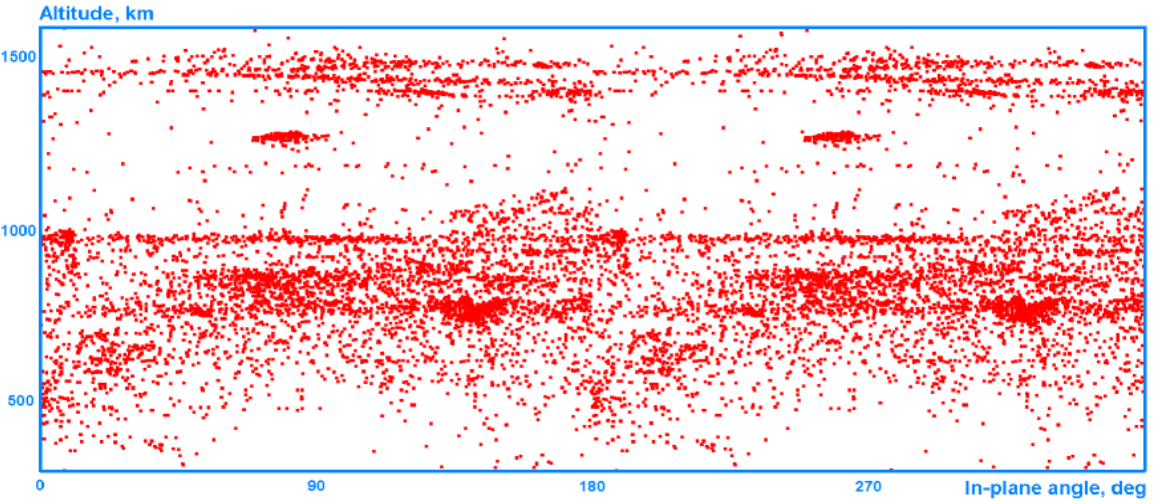
\includegraphics[width=0.8\textwidth]{figures/TrackedObjectsCrossingSCOrbitalPlane.png}
    \caption{Tracked Objects Crossing the Orbital Plane of a Spacecraft in LEO}
    \label{fig:ObjectsCrossing_SC_OP}
\end{figure}

\begin{itemize}
  \item One problem with the LEO catalog is that the accuracy of predictions of the future location of objects in LEO is not always good. Because of this, the use of the LEO catalog as a collision avoidance tool is not always practical [2].
  \item Function spacecraft represents only about one fifth.[3]
\end{itemize}


%\begin{center}
%    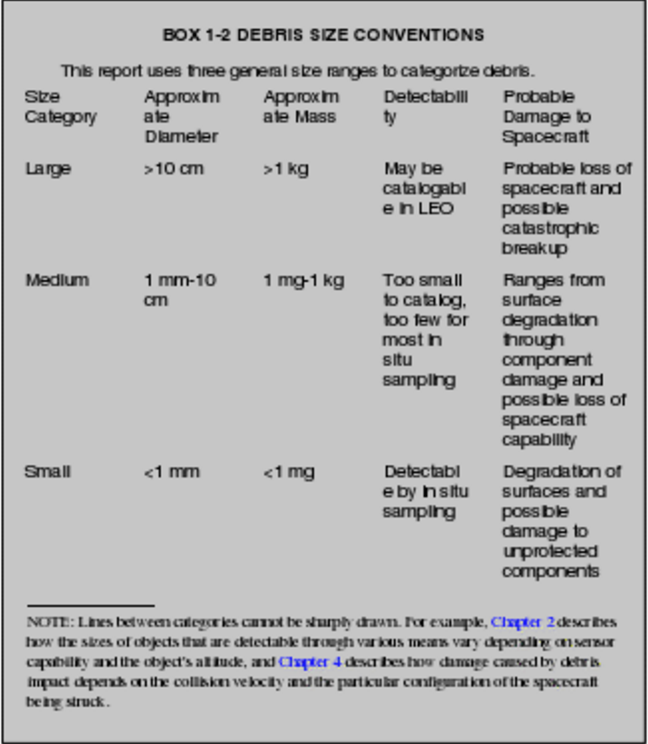
\includegraphics[]{figures/DebrisSizingChart.png}
%\end{center}
%\caption{Debris sizing chart.}\label{Fig:sizingChart}



\clearpage

\bibliographystyle{unsrt}
\bibliography{FelipeResearch}


\end{document}




